\documentclass{standalone}
% Shared figure style: the paper's typefaces, sizes and the two-colour encoding.
% Identical copies live in every figure directory so that each builds on its own.
\usepackage{fontspec}
\setmainfont{LinLibertine}[Extension=.otf,UprightFont=*_R,ItalicFont=*_RI,BoldFont=*_RB]
\setsansfont{LinBiolinum}[Extension=.otf,UprightFont=*_R,ItalicFont=*_RI,BoldFont=*_RB]
\usepackage{unicode-math}
\setmathfont{LibertinusMath-Regular.otf}
\setmathfont{LinLibertine_R.otf}[range=up/num]
% Sub- and superscripts (R_1, t^*, 10^{-4}) at 6 pt, so no glyph is below 6 pt.
\DeclareMathSizes{7}{7}{6}{6}
\DeclareMathSizes{7.5}{7.5}{6}{6}
\DeclareMathSizes{8}{8}{6}{6}
\usepackage{tikz}
\usetikzlibrary{patterns.meta,calc,arrows.meta}
\usepackage{pgfplots}
\pgfplotsset{compat=1.18}
% Blue: what a sound field proves (certain presence, revision IDs).
% Red: the inference that fails (equal reusable fields, content hashes).
\definecolor{sound}{HTML}{2166AC}
\definecolor{fails}{HTML}{B2182B}
\definecolor{ink}{HTML}{1A1A1A}
\definecolor{muted}{HTML}{5C5C5C}
\definecolor{rule}{HTML}{8A8A8A}
\newcommand{\figtitle}{\fontsize{8}{9.6}\selectfont}
\newcommand{\figlabel}{\fontsize{7.5}{9}\selectfont}
\newcommand{\figsmall}{\fontsize{7}{8.4}\selectfont}

\begin{document}
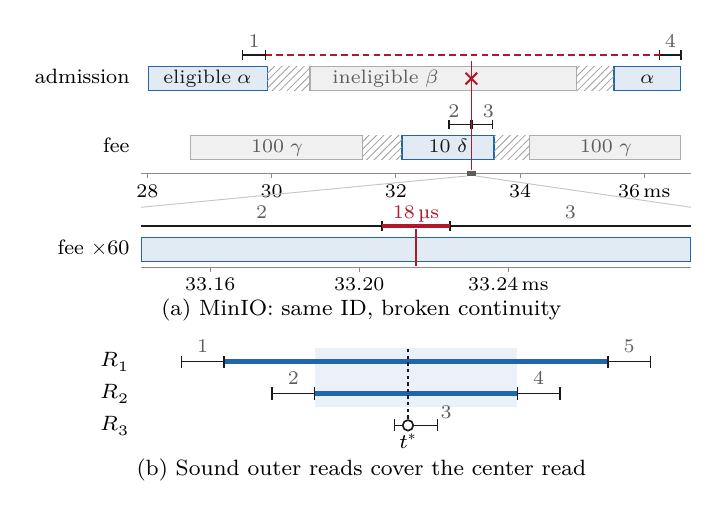
\begin{tikzpicture}[x=1pt, y=1pt]
\useasboundingbox (0,-164.90) rectangle (241.15,0);
\filldraw[fill=sound!13, draw=sound, line width=0.4pt] (43.59,-22.70) rectangle (86.56,-14.10);
\node[font=\figsmall, text=ink, inner sep=0pt] at (65.07,-18.40) {\strut eligible\,\,$\alpha$};
\filldraw[fill=black!6, draw=black!32, line width=0.4pt] (102.02,-22.70) rectangle (198.39,-14.10);
\node[font=\figsmall, text=muted, inner sep=0pt] at (129.16,-18.40) {\strut ineligible\,\,$\beta$};
\filldraw[fill=sound!13, draw=sound, line width=0.4pt] (211.86,-22.70) rectangle (236.05,-14.10);
\node[font=\figsmall, text=ink, inner sep=0pt] at (223.95,-18.40) {\strut $\alpha$};
\filldraw[fill=black!6, draw=black!32, line width=0.4pt] (58.88,-47.70) rectangle (121.03,-39.10);
\node[font=\figsmall, text=muted, inner sep=0pt] at (89.96,-43.40) {\strut 100\,\,$\gamma$};
\filldraw[fill=sound!13, draw=sound, line width=0.4pt] (135.25,-47.70) rectangle (168.51,-39.10);
\node[font=\figsmall, text=ink, inner sep=0pt] at (151.88,-43.40) {\strut 10\,\,$\delta$};
\filldraw[fill=black!6, draw=black!32, line width=0.4pt] (181.49,-47.70) rectangle (236.05,-39.10);
\node[font=\figsmall, text=muted, inner sep=0pt] at (208.77,-43.40) {\strut 100\,\,$\gamma$};
\fill[pattern={Lines[angle=45,distance=1.9pt,line width=0.3pt]}, pattern color=black!38] (86.56,-22.70) rectangle (102.02,-14.10);
\fill[pattern={Lines[angle=45,distance=1.9pt,line width=0.3pt]}, pattern color=black!38] (198.39,-22.70) rectangle (211.86,-14.10);
\fill[pattern={Lines[angle=45,distance=1.9pt,line width=0.3pt]}, pattern color=black!38] (121.03,-47.70) rectangle (135.25,-39.10);
\fill[pattern={Lines[angle=45,distance=1.9pt,line width=0.3pt]}, pattern color=black!38] (168.51,-47.70) rectangle (181.49,-39.10);
\draw[ink, line width=0.5pt] (77.58,-9.90) -- (86.00,-9.90);
\draw[ink, line width=0.5pt] (77.58,-11.60) -- (77.58,-8.20);
\draw[ink, line width=0.5pt] (86.00,-11.60) -- (86.00,-8.20);
\node[font=\figsmall, text=muted, anchor=base, inner sep=0pt] at (81.79,-7.30) {1};
\draw[ink, line width=0.5pt] (152.25,-34.90) -- (160.10,-34.90);
\draw[ink, line width=0.5pt] (152.25,-36.60) -- (152.25,-33.20);
\draw[ink, line width=0.5pt] (160.10,-36.60) -- (160.10,-33.20);
\node[font=\figsmall, text=muted, anchor=base, inner sep=0pt] at (153.97,-32.30) {2};
\draw[ink, line width=0.5pt] (160.51,-34.90) -- (168.00,-34.90);
\draw[ink, line width=0.5pt] (160.51,-36.60) -- (160.51,-33.20);
\draw[ink, line width=0.5pt] (168.00,-36.60) -- (168.00,-33.20);
\node[font=\figsmall, text=muted, anchor=base, inner sep=0pt] at (166.46,-32.30) {3};
\draw[ink, line width=0.5pt] (228.36,-9.90) -- (236.05,-9.90);
\draw[ink, line width=0.5pt] (228.36,-11.60) -- (228.36,-8.20);
\draw[ink, line width=0.5pt] (236.05,-11.60) -- (236.05,-8.20);
\node[font=\figsmall, text=muted, anchor=base, inner sep=0pt] at (232.20,-7.30) {4};
\draw[fails, line width=0.6pt, dash pattern=on 2.4pt off 1.5pt] (86.00,-9.90) -- (228.36,-9.90);
\draw[fails, line width=0.5pt] (160.31,-51.50) -- (160.31,-12.10);
\draw[fails, line width=0.75pt] (158.21,-20.50) -- (162.41,-16.30) (158.21,-16.30) -- (162.41,-20.50);
\node[font=\figlabel, anchor=east, inner sep=0pt] at (37.00,-18.40) {\strut admission};
\node[font=\figlabel, anchor=east, inner sep=0pt] at (37.00,-43.40) {\strut fee};
\draw[rule, line width=0.4pt] (41.00,-52.70) -- (239.65,-52.70);
\draw[rule, line width=0.4pt] (43.24,-52.70) -- (43.24,-54.50);
\node[font=\figsmall, anchor=base, inner sep=0pt] at (43.24,-61.30) {28};
\draw[rule, line width=0.4pt] (88.14,-52.70) -- (88.14,-54.50);
\node[font=\figsmall, anchor=base, inner sep=0pt] at (88.14,-61.30) {30};
\draw[rule, line width=0.4pt] (133.03,-52.70) -- (133.03,-54.50);
\node[font=\figsmall, anchor=base, inner sep=0pt] at (133.03,-61.30) {32};
\draw[rule, line width=0.4pt] (177.92,-52.70) -- (177.92,-54.50);
\node[font=\figsmall, anchor=base, inner sep=0pt] at (177.92,-61.30) {34};
\draw[rule, line width=0.4pt] (222.81,-52.70) -- (222.81,-54.50);
\node[font=\figsmall, anchor=base, inner sep=0pt] at (222.81,-61.30) {36\,ms};
\fill[muted] (158.65,-53.60) rectangle (161.96,-51.80);
\draw[black!22, line width=0.35pt] (158.65,-53.60) -- (41.00,-64.90) (161.96,-53.60) -- (239.65,-64.90);
\filldraw[fill=sound!13, draw=sound, line width=0.4pt] (41.00,-84.50) rectangle (239.65,-75.90);
\draw[ink, line width=0.5pt] (41.00,-71.70) -- (128.09,-71.70);
\draw[ink, line width=0.5pt] (128.09,-73.40) -- (128.09,-70.00);
\node[font=\figsmall, text=muted, anchor=base, inner sep=0pt] at (84.55,-69.10) {2};
\draw[ink, line width=0.5pt] (152.56,-71.70) -- (239.65,-71.70);
\draw[ink, line width=0.5pt] (152.56,-73.40) -- (152.56,-70.00);
\node[font=\figsmall, text=muted, anchor=base, inner sep=0pt] at (196.10,-69.10) {3};
\draw[fails, line width=1.6pt] (128.09,-71.70) -- (152.56,-71.70);
\draw[fails, line width=0.5pt] (140.32,-86.00) -- (140.32,-72.70);
\node[font=\figsmall, text=fails, anchor=base, inner sep=0pt] at (140.32,-69.10) {18\,µs};
\node[font=\figlabel, anchor=east, inner sep=0pt] at (37.00,-80.20) {\strut fee $\times$60};
\draw[rule, line width=0.4pt] (41.00,-86.50) -- (239.65,-86.50);
\draw[rule, line width=0.4pt] (65.97,-86.50) -- (65.97,-88.30);
\node[font=\figsmall, anchor=base, inner sep=0pt] at (65.97,-95.10) {33.16};
\draw[rule, line width=0.4pt] (119.84,-86.50) -- (119.84,-88.30);
\node[font=\figsmall, anchor=base, inner sep=0pt] at (119.84,-95.10) {33.20};
\draw[rule, line width=0.4pt] (173.71,-86.50) -- (173.71,-88.30);
\node[font=\figsmall, anchor=base, inner sep=0pt] at (173.71,-95.10) {33.24\,ms};
\node[font=\figtitle, anchor=base, inner sep=0pt] at (120.57,-104.10) {(a) MinIO: same ID, broken continuity};
\fill[sound!9] (103.72,-137.20) rectangle (176.93,-115.70);
\draw[sound, line width=2.0pt] (70.97,-120.70) -- (209.68,-120.70);
\draw[sound, line width=2.0pt] (103.72,-132.20) -- (176.93,-132.20);
\draw[ink, line width=0.5pt] (55.56,-120.70) -- (70.97,-120.70);
\draw[ink, line width=0.5pt] (55.56,-122.90) -- (55.56,-118.50);
\draw[ink, line width=0.5pt] (70.97,-122.90) -- (70.97,-118.50);
\node[font=\figsmall, text=muted, anchor=base, inner sep=0pt] at (63.26,-117.30) {1};
\draw[ink, line width=0.5pt] (88.31,-132.20) -- (103.72,-132.20);
\draw[ink, line width=0.5pt] (88.31,-134.40) -- (88.31,-130.00);
\draw[ink, line width=0.5pt] (103.72,-134.40) -- (103.72,-130.00);
\node[font=\figsmall, text=muted, anchor=base, inner sep=0pt] at (96.01,-128.80) {2};
\draw[ink, line width=0.5pt] (132.62,-143.70) -- (148.03,-143.70);
\draw[ink, line width=0.5pt] (132.62,-145.90) -- (132.62,-141.50);
\draw[ink, line width=0.5pt] (148.03,-145.90) -- (148.03,-141.50);
\node[font=\figsmall, text=muted, anchor=base, inner sep=0pt] at (151.23,-141.30) {3};
\draw[ink, line width=0.5pt] (176.93,-132.20) -- (192.34,-132.20);
\draw[ink, line width=0.5pt] (176.93,-134.40) -- (176.93,-130.00);
\draw[ink, line width=0.5pt] (192.34,-134.40) -- (192.34,-130.00);
\node[font=\figsmall, text=muted, anchor=base, inner sep=0pt] at (184.63,-128.80) {4};
\draw[ink, line width=0.5pt] (209.68,-120.70) -- (225.09,-120.70);
\draw[ink, line width=0.5pt] (209.68,-122.90) -- (209.68,-118.50);
\draw[ink, line width=0.5pt] (225.09,-122.90) -- (225.09,-118.50);
\node[font=\figsmall, text=muted, anchor=base, inner sep=0pt] at (217.38,-117.30) {5};
\draw[ink, line width=0.45pt, dash pattern=on 1.2pt off 1.2pt] (137.43,-141.30) -- (137.43,-115.70);
\filldraw[fill=white, draw=ink, line width=0.6pt] (137.43,-143.70) circle (1.9pt);
\node[font=\figlabel, anchor=north, inner sep=0pt] at (137.43,-146.70) {$t^{*}$};
\node[font=\figlabel, anchor=east, inner sep=0pt] at (37.00,-120.70) {\strut $R_1$};
\node[font=\figlabel, anchor=east, inner sep=0pt] at (37.00,-132.20) {\strut $R_2$};
\node[font=\figlabel, anchor=east, inner sep=0pt] at (37.00,-143.70) {\strut $R_3$};
\node[font=\figtitle, anchor=base, inner sep=0pt] at (120.57,-161.70) {(b) Sound outer reads cover the center read};
\end{tikzpicture}
\end{document}
